\chapter{Resultados}
\label{chapter:resultados}

\section{Análisis de Rendimiento}

Es importante realizar el análisis de rendimiento de una aplicación distribuida con el propósito de estudiar los beneficios que ésta posee ante la comparación con su versión secuencial. 
Al desarrollar un programa distribuido no solo se intenta alcanzar el mejor rendimiento del mismo sino que también se intenta mantenerlo en proporción, a medida que se añaden nuevos nodos de procesamiento.

En el caso de una aplicación secuencial, ésta es usualmente evaluada en términos de su tiempo de ejecución expresado como una función de su tamaño de entrada. El tiempo de ejecución de un programa distribuido no sólo es evaluado en términos del tamaño de la entrada sino que también influyen otros factores tales como el número de nodos de procesamiento que posee y el coste de comunicación entre dichos nodos.

A continuación se muestra el análisis de rendimiento de la aplicación Parallel-Clusterer en términos de las métricas principales calculadas sobre este programa, tales como  \textit{aceleración, eficiencia, overhead} y \textit{costo}. La ejecución se llevo a cabo con un archivo de entrada generado con 9 residuos, variando de 1 a 5 clientes conectados.\\

\subsection{Tiempo de ejecución}

El tiempo de ejecución de un programa se define como el intervalo de tiempo que transcurre desde que el programa se inicia hasta que finaliza. En el caso de un programa distribuido, éste se calcula desde que se inicia el mismo hasta que el último nodo finaliza su ejecución.

Se denotará el tiempo secuencial que toma la aplicación como \textit{T$_{s}$} y el tiempo distribuido como \textit{T$_{p}$}. El promedio de \textit{T$_{s}$} luego de 10 ejecuciones de la aplicación Parallel-Clusterer fue de 110.7 segundos.

En la figura \ref{ts_vs_tp} se muestran los tiempos de ejecución promedio para cinco clientes así como su comparación con el algoritmo secuencial. Podemos observar sobre dicha figura que, con solo 5 nodos, los tiempos de procesamiento que toma la solución distribuida no es más óptima respecto de la solución secuencial. Sin embargo, es fácil ver que el tiempo va disminuyendo considerablemente a medida que se agregan nodos de procesamiento. Estos resultados variaron por diversos factores más allá del coste de comunicación y de la cantidad de nodos:

\begin{itemize}

  \item \textit{descarga de trabajos:} los trabajos de entrada que recibe cada cliente pesaron entre 60kb y 390kb. El tiempo tomado por cada cliente en descargar los trabajos en relación con su velocidad de conexión obviamente afectó directamente al tiempo total de la aplicación.

  \item \textit{subir resultados al servidor:} los resultados generados son escritos en un archivo de salida para que luego cada cliente BOINC los suba al servidor del proyecto. En este caso, el tiempo que tardó un cliente en subir dicho archivo, en relación con su velocidad de conexión, influyó también en el tiempo total de la aplicación.

  \item \textit{tiempo entre requerimientos:} la aplicación \textit{BOINC Manager}, nombrada en la sección \ref{boinc:manager}, envía requerimientos de nuevas tareas al servidor cada X cantidad de tiempo (X representa segundos e incluso minutos). Por ejemplo, en estas pruebas, el cliente envió requerimientos al servidor instantáneamente después de reportar una tarea. Si mediante éstos no obtuvo nuevos trabajos, esperaba entre 1 y 2 minutos para volver a requerir. Esto último es un factor negativo para el tiempo final.

\end{itemize}
\label{factores:tiempo}

\begin{center}
\begin{figure}[!ht]
    %Tabla & Grafico
    \begin{minipage}{2,5cm}
    \begin{flushleft}
    \begin{tabular*}{2,0cm}{c@{\extracolsep{\fill}}c}
        \hline
        \textbf{p} & \textbf{$T_p$} \\ \hline 
        1 & 305 \\ \hline
        2 & 249 \\ \hline
        3 & 259 \\ \hline
        4 & 245 \\ \hline
        5 & 222 \\ \hline
    \end{tabular*}
    \end{flushleft}
    \end{minipage}
    \    \ \hfill
    \begin{minipage}{12cm}
    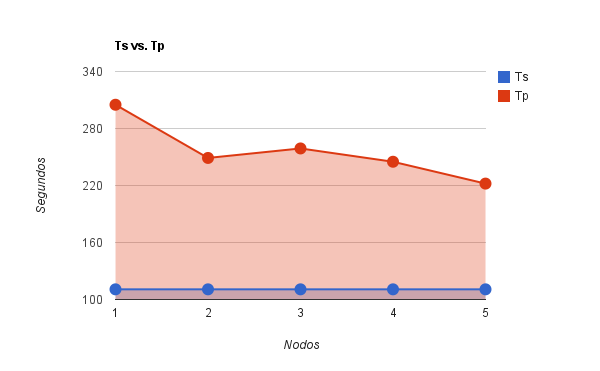
\includegraphics[scale=0.6]{images/Grafico_de_tiempos.png}\\
    \end{minipage}
    \caption{Tiempo secuencial vs. paralelo}
    \label{ts_vs_tp}
\end{figure}
\end{center}

Haciendo un análisis de la comparación que se observa en el gráfico \ref{ts_vs_tp}, y considerando que las \texttt{JobUnits} generadas por la aplicación en estas pruebas pesaron como máximo aproximada \texttt{400kb}, se podría pensar en una nueva versión del Parallel-Clusterer pensada para trabajar con FuD-BOINC en donde cada \texttt{JobUnit} demore mucho más en procesarse aumentando la cantidad de instrucciones efectuadas por un cliente con el fin de reducir la cantidad de requerimientos generados por los clientes.


\subsection{Aceleración}

Es una medida que arroja el beneficio relativo de resolver un problema en paralelo. Ésta es definida como la relación del tiempo que toma resolver un problema en un sólo procesador con el tiempo requerido para resolverlo en una arquitectura paralela con \textit{n} nodos de procesamiento idénticos. Se denota con el símbolo \textit{S} y se define como
\textit{S} = \textit{T$_{s}$}/\textit{T$_{p}$}

\begin{center}
\begin{figure}[!ht]
    %Tabla & Grafico
    \begin{minipage}{2,5cm}
    \begin{flushleft}
    \begin{tabular*}{2,0cm}{c@{\extracolsep{\fill}}c}
        \hline
        \textbf{p} & \textbf{$S$} \\ \hline 
        1  & 0.36 \\ \hline
        2  & 0.44 \\ \hline
        3  & 0.42 \\ \hline
        4  & 0.45 \\ \hline
        5  & 0.49 \\ \hline
    \end{tabular*}
    \end{flushleft}
    \end{minipage}
    \    \ \hfill
    \begin{minipage}{12cm}
    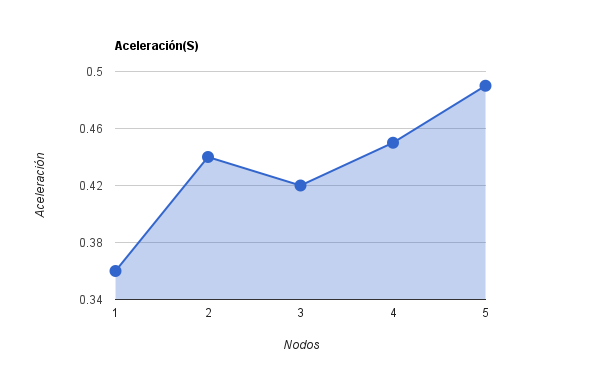
\includegraphics[scale=0.6]{images/Grafico_Aceleracion.png}\\
    \end{minipage}
    \caption{Aceleración}
    \label{speedup}
\end{figure}
\end{center}

En la figura \ref{speedup} podemos observar que no hay un crecimiento ``lineal'' de la aceleración. Se puede ver que para 2 nodos la aceleración mejora respecto del valor obtenido con 3 nodos. Este caso se debe a los factores explicados anteriormente, donde evidentemente en la ejecución con 3 nodos afectaron más que en el resto de los casos. Sacando ese caso particular, se observa que la aceleración crece a medida que se agregan más nodos de procesamiento. Ésto se debe a que al aumentar la cantidad de nodos disponibles, aumenta la cantidad de requerimientos provocando que las tareas sean asignadas más rápido a los clientes.

\subsection{Eficiencia}

La eficiencia de un programa paralelo indica la fracción de tiempo útil de un elemento de procesamiento. 
Se define como: \textit{E} = \textit{S}/\textit{p}

\begin{center}
\begin{figure}[H]
    %Tabla & Grafico
    \begin{minipage}{2,5cm}
    \begin{flushleft}
    \begin{tabular*}{2,0cm}{c@{\extracolsep{\fill}}c}
        \hline
        \textbf{p} & \textbf{$E$} \\ \hline 
        1  & 0.36 \\ \hline
        2  & 0,22 \\ \hline
        3  & 0,14 \\ \hline
        4  & 0,11 \\ \hline
        5  & 0,09 \\ \hline
    \end{tabular*}
    \end{flushleft}
    \end{minipage}
    \    \ \hfill
    \begin{minipage}{12cm}
    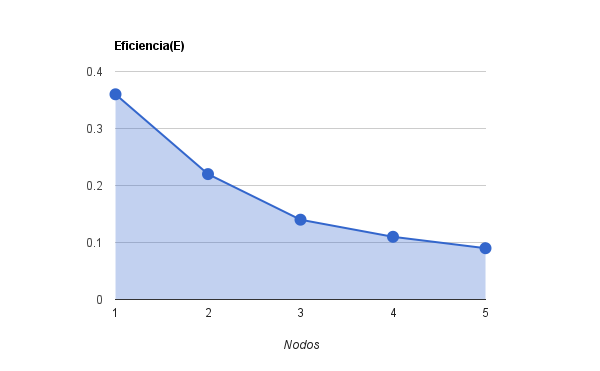
\includegraphics[scale=0.5]{images/Grafico_Eficiencia.png}\\
    \end{minipage}
    \caption{Eficiencia}
    \label{eficiency}
\end{figure}
\end{center}

En la figura \ref{eficiency}, vemos que la función de eficiencia decae, lo que significa una utilidad nodal inversamente proporcional a la cantidad de nodos de procesamiento. Ésto deja en claro que a mayor cantidad de nodos, más decae la eficiencia.


\subsection{Overhead}

El overhead de un programa paralelo es el trabajo adicional que dicho programa realiza respecto a la solución secuencial equivalente y se define como:

\textit{T$_{o}$} = \textit{p} ∗ \textit{T$_{p}$} − \textit{T$_{s}$}

\begin{center}
\begin{figure}[H]
    %Tabla & Grafico
    \begin{minipage}{2,5cm}
    \begin{flushleft}
    \begin{tabular*}{2,0cm}{c@{\extracolsep{\fill}}c}
        \hline
        \textbf{p} & \textbf{$T_0$} \\ \hline 
        1  & 194.3 \\ \hline
        2  & 387.3 \\ \hline
        3  & 666.3 \\ \hline
        4  & 869.3 \\ \hline
        5  & 999.3 \\ \hline
    \end{tabular*}
    \end{flushleft}
    \end{minipage}
    \    \ \hfill
    \begin{minipage}{12cm}
    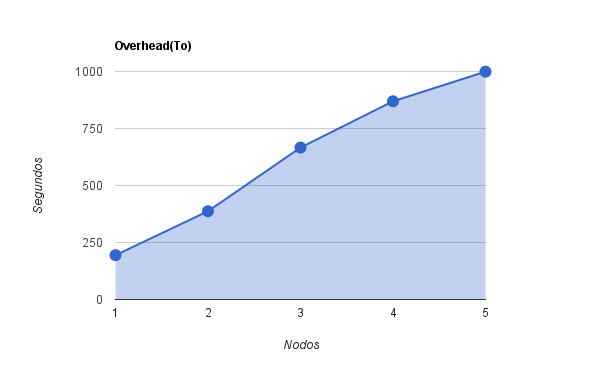
\includegraphics[scale=0.6]{images/Grafico_Overhead.png}\\
    \end{minipage}
    \caption{Overhead}
    \label{overhead}
\end{figure}
\end{center}

En la figura \ref{overhead}, vemos que el overhead aumenta a medida que se agregan nodos de procesamiento, lo que indica una suma de trabajo adicional por cada nuevo nodo de procesamiento. En el caso de FuD-BOINC, este trabajo adicional que agrega cada cliente se debe a un aumento de la cantidad de requerimientos que debe atender el servidor.

\subsection{Costo}

El costo de un programa paralelo refleja la suma de los tiempos de ejecución de cada proceso, y se define como:
 \textit{C} = \textit{p} ∗ \textit{T$_{p}$} . Se dice que un programa paralelo tiene costo óptimo si tiene costo computacional igual al programa secuencial.

\newpage
\begin{center}
\begin{figure}[!ht]
    \begin{minipage}{2,5cm}
    \begin{flushleft}
    \begin{tabular*}{2,0cm}{c@{\extracolsep{\fill}}c}
        \hline
        \textbf{p} & \textbf{$C$} \\ \hline 
        1  & 305 \\ \hline
        2  & 498 \\ \hline
        3  & 777 \\ \hline
        4  & 980 \\ \hline
        5  & 1110 \\ \hline
    \end{tabular*}
    \end{flushleft}
    \end{minipage}
    \    \ \hfill
    \begin{minipage}{12cm}
    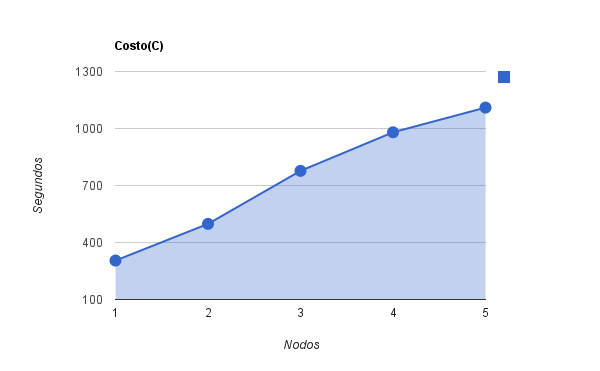
\includegraphics[scale=0.6]{images/Grafico_Costo.png}\\
    \end{minipage}
    \caption{Costo}
    \label{cost}
\end{figure}
\end{center}

En la figura \ref{cost} se observa que el costo tiene una curva similar al overhead. En este gráfico se muestra un costo directamente proporcional a la cantidad de nodos participantes.

\section{FuD-BOINC Vs FuD-Asio}

En esta sección se presenta una comparación de los resultados obtenidos de ejecutar la aplicación Parallel-Clusterer (\ref{seccion:pruebas:clusterer}) compilada con las librerías FuD-BOINC y FuD original (FuD-Asio). El objetivo de esta comparación consiste en poder verificar que los resultados de ambas pruebas sean iguales o aproximados con el fin de poder contar con resultados que garanticen que el diseño e implementación de FuD-BOINC siguen manteniendo el modelo que ofrece el diseño de original de FuD.

Debemos destacar que dicha aplicación genera resultados no determinísticos. Ésto se debe a la forma en que se eligen los representantes de cada clúster resultante. Por ejemplo, al principio de la computación se envían a los clientes \texttt{JobUnits} para armar un conjunto de representantes a partir de los cuales se van a construir los clusters. En cada ejecución, podría ocurrir que los clientes retornen los resultados\footnote{Un representante para la creación de un clúster} en distinto orden respecto del \texttt{ID} que posee la \texttt{JobUnit} asignada a cada uno. De esta manera, los resultados finales  podrían variar por cada ejecución ya que los representantes utilizados para comenzar a crear cada clúster podrían llegar en distinto orden. \\

Para la obtención de resultados, se tomaron como casos de prueba la ejecución de la aplicación Parallel-Clusterer pasándole como entrada archivos generados con 5,6,7,8 y 9 residuos comparando la cantidad de clusters obtenidos. El cuadro \ref{Fb_vs_fa} muestra los valores obtenido por cada ejecución. La columna \textit{residuos} indica la cantidad de residuos con los que se generó el archivo de entrada que se utilizó para esa prueba. Las columnas \textit{``N° Clusters con FuD-BOINC''} y \textit{``N° Clusters con FuD-Asio''} muestran la cantidad de clústers obtenidos en la ejecución de la aplicación utilizando la librería FuD-BOINC y FuD-Asio respectivamente.\\

\begin{table}[H]
\begin{center}
\begin{tabular}{| c| c| c| c|}
\hline
\textbf{Residuos} & \textbf{N° Clusters con FuD-BOINC} & \textbf{N° Clusters con FuD-Asio}\\ \hline 
5  & 11 & 11 \\ 
\hline
6  & 50 & 50 \\ 
\hline
7  & 155 & 155 \\ 
\hline
8  & 384 & 384 \\ 
\hline
9  & 1023 & 1023 \\ 
\hline
\end{tabular}
\caption{Comparación de resultados Parallel-Clusterer}
\label{Fb_vs_fa}
\end{center}
\end{table}

Considerando que las pruebas se realizaron utilizando una aplicación compleja como es el Parallel-Clusterer y que en los resultados plasmados en el cuadro \ref{Fb_vs_fa} la cantidad de clústers obtenidos son equivalentes en todas las pruebas realizadas, se puede decir que el comportamiento de dicha aplicación utilizando la capa de distribución FuD-BOINC fue el esperado.